\section{Approach}

% FPs to SLOCs:
% using table from http://www.qsm.com/resources/function-point-languages-table
%           VV
% 111 FPs * 46 = 5106 SLOCs
In order to apply the COCOMOII method, we apply first a simple \textit{Funtion Points to Lines Of Code}
conversion. The adjustment factor of 46 is provided by the updated table available at 
http://www.qsm.com/resources/function-point-languages-table
\begin{equation}
 111 \text{ FPs} * 46 = 5106 \text{ SLOCs}
\end{equation}

%effort=2.94*EAF*(KLOC)^E
The effort estimation takes into account a ``Nominal'' value for all the Cost Drivers and Scale Drivers.
\begin{multline}
 \text{effort} = 2.94 * \textit{EAF} * (\textit{KLOC})^E \\
 \textit{EAF} = 1.0 \\
 \textit{KLOC} = 5.106 \\
 E = 1.0997 \\
 \text{Therefore, effort} = 2.94 * 1.0 * (5.106)^{1.0997} = 17.66 \text{ Person/Months} \\
\end{multline}

%duration=3.67*(effort)^Se
Next, we estimate the project duration using the following equation.
\begin{multline}
 \text{duration} = 3.67 * (\textit{effort})^\textit{Se} \\
 \textit{Se} = 0.3179 \\
 \text{Therefore, duration} = 3.67 * (17.66)^{0.3179} = 9.14 \text{ Months} \\
\end{multline}

%Npeople=effort/duration
Last, we determine the number of people required to complete the project within
the previously computed parameters
\begin{multline}
 N_{\textit{people}} = \lceil \textit{effort} / \textit{duration} \rceil \\
 \textit{Se} = 0.3179 \\
 \text{Therefore, } N_{\textit{people}} = \lceil 17.66 / 9.14 \rceil = 2 \text{ People} \\
\end{multline}
% we'll just call them 'Alice' and 'Bob'

\section{Results}
We employed an online COCOMOII calculator in order to generate a more fine-grained estimate. \\
The following results were obtained using the tool available at \\
http://csse.usc.edu/tools/COCOMOII.php \\

\subsection{Input (software sizing)}
\begin{longtable}[c]{@{}llllllll@{}}
\toprule
\begin{minipage}[t]{0.10\columnwidth}\raggedright\strut
\strut\end{minipage} &
\begin{minipage}[t]{0.10\columnwidth}\raggedright\strut
\href{http://sunset.usc.edu/research/COCOMOII/expert_cocomo/sloc.html}{SLOC}
\strut\end{minipage} &
\begin{minipage}[t]{0.10\columnwidth}\raggedright\strut
\emph{~}\% Design Modified
\strut\end{minipage} &
\begin{minipage}[t]{0.10\columnwidth}\raggedright\strut
\% Code Modified
\strut\end{minipage} &
\begin{minipage}[t]{0.10\columnwidth}\raggedright\strut
\% Integration Required
\strut\end{minipage} &
\begin{minipage}[t]{0.10\columnwidth}\raggedright\strut
Assessment and Assimilation\\
(0\% - 8\%)
\strut\end{minipage} &
\begin{minipage}[t]{0.10\columnwidth}\raggedright\strut
~Software Understanding\\
(0\% - 50\%)
\strut\end{minipage} &
\begin{minipage}[t]{0.10\columnwidth}\raggedright\strut
Unfamiliarity\\
(0-1)
\strut\end{minipage}\tabularnewline
\begin{minipage}[t]{0.10\columnwidth}\raggedright\strut
New\\
\strut\end{minipage} &
\begin{minipage}[t]{0.10\columnwidth}\raggedright\strut
5106
\strut\end{minipage} &
\begin{minipage}[t]{0.10\columnwidth}\raggedright\strut
\strut\end{minipage} &
\begin{minipage}[t]{0.10\columnwidth}\raggedright\strut
\strut\end{minipage} &
\begin{minipage}[t]{0.10\columnwidth}\raggedright\strut
\strut\end{minipage} &
\begin{minipage}[t]{0.10\columnwidth}\raggedright\strut
\strut\end{minipage} &
\begin{minipage}[t]{0.10\columnwidth}\raggedright\strut
\strut\end{minipage} &
\begin{minipage}[t]{0.10\columnwidth}\raggedright\strut
\strut\end{minipage}\tabularnewline
\begin{minipage}[t]{0.10\columnwidth}\raggedright\strut
Reused\\
\strut\end{minipage} &
\begin{minipage}[t]{0.10\columnwidth}\raggedright\strut
\strut\end{minipage} &
\begin{minipage}[t]{0.10\columnwidth}\raggedright\strut
0
\strut\end{minipage} &
\begin{minipage}[t]{0.10\columnwidth}\raggedright\strut
0
\strut\end{minipage} &
\begin{minipage}[t]{0.10\columnwidth}\raggedright\strut
\strut\end{minipage} &
\begin{minipage}[t]{0.10\columnwidth}\raggedright\strut
\strut\end{minipage} &
\begin{minipage}[t]{0.10\columnwidth}\raggedright\strut
\strut\end{minipage} &
\begin{minipage}[t]{0.10\columnwidth}\raggedright\strut
\strut\end{minipage}\tabularnewline
\begin{minipage}[t]{0.10\columnwidth}\raggedright\strut
Modified\\
\strut\end{minipage} &
\begin{minipage}[t]{0.10\columnwidth}\raggedright\strut
\strut\end{minipage} &
\begin{minipage}[t]{0.10\columnwidth}\raggedright\strut
\strut\end{minipage} &
\begin{minipage}[t]{0.10\columnwidth}\raggedright\strut
\strut\end{minipage} &
\begin{minipage}[t]{0.10\columnwidth}\raggedright\strut
\strut\end{minipage} &
\begin{minipage}[t]{0.10\columnwidth}\raggedright\strut
\strut\end{minipage} &
\begin{minipage}[t]{0.10\columnwidth}\raggedright\strut
\strut\end{minipage} &
\begin{minipage}[t]{0.10\columnwidth}\raggedright\strut
\strut\end{minipage}\tabularnewline
\bottomrule
\end{longtable}


\subsection{Input (drivers)}
\begin{description}
\item [Precedentedness:] Nominal
\item [Development Flexibility:] Nominal
\item [Required Software Reliability:] Nominal
\item [Data Base Size:] Nominal
\item [Product Complexity:] Nominal
\item [Developed for Reusability:] Nominal
\item [Documentation Match to Lifecycle Needs:] Nominal
\item [Architecture / Risk Resolution:] Nominal
\item [Team Cohesion:] Nominal
\item [Analyst Capability:] Nominal
\item [Programmer Capability:] Nominal
\item [Personnel Continuity:] Nominal
\item [Application Experience:] Nominal
\item [Platform Experience:] Nominal
\item [Language and Toolset Experience:] Nominal
\item [Process Maturity:] Nominal
\item [Time Constraint:] Nominal
\item [Storage Constraint:] Nominal
\item [Platform Volatility:] Nominal
\item [Use of Software Tools:] Nominal
\item [Multisite Development:] Nominal
\item [Required Development Schedule:] Nominal
\end{description}


We'll also assume a cost per Person-Month of 2000\$

\subsection{Output}

\textit{(dummy-data)}

\textbf{Software Development (Elaboration and
Construction)}\\[2\baselineskip]Effort = 18.1 Person-months\\
Schedule = 9.5 Months\\
Cost = \$27160\\[2\baselineskip]Total Equivalent Size =
5223~SLOC\\[2\baselineskip]\textbf{Acquisition Phase Distribution}\\
{ }

\begin{longtable}[c]{@{}lllll@{}}
\toprule
\begin{minipage}[t]{0.17\columnwidth}\raggedright\strut
Phase
\strut\end{minipage} &
\begin{minipage}[t]{0.17\columnwidth}\raggedright\strut
Effort (Person-months)
\strut\end{minipage} &
\begin{minipage}[t]{0.17\columnwidth}\raggedright\strut
Schedule (Months)
\strut\end{minipage} &
\begin{minipage}[t]{0.17\columnwidth}\raggedright\strut
Average Staff
\strut\end{minipage} &
\begin{minipage}[t]{0.17\columnwidth}\raggedright\strut
Cost (Dollars)
\strut\end{minipage}\tabularnewline
\begin{minipage}[t]{0.17\columnwidth}\raggedright\strut
Inception
\strut\end{minipage} &
\begin{minipage}[t]{0.17\columnwidth}\raggedright\strut
1.1
\strut\end{minipage} &
\begin{minipage}[t]{0.17\columnwidth}\raggedright\strut
1.2
\strut\end{minipage} &
\begin{minipage}[t]{0.17\columnwidth}\raggedright\strut
0.9
\strut\end{minipage} &
\begin{minipage}[t]{0.17\columnwidth}\raggedright\strut
\$1630
\strut\end{minipage}\tabularnewline
\begin{minipage}[t]{0.17\columnwidth}\raggedright\strut
Elaboration
\strut\end{minipage} &
\begin{minipage}[t]{0.17\columnwidth}\raggedright\strut
4.3
\strut\end{minipage} &
\begin{minipage}[t]{0.17\columnwidth}\raggedright\strut
3.6
\strut\end{minipage} &
\begin{minipage}[t]{0.17\columnwidth}\raggedright\strut
1.2
\strut\end{minipage} &
\begin{minipage}[t]{0.17\columnwidth}\raggedright\strut
\$6518
\strut\end{minipage}\tabularnewline
\begin{minipage}[t]{0.17\columnwidth}\raggedright\strut
Construction
\strut\end{minipage} &
\begin{minipage}[t]{0.17\columnwidth}\raggedright\strut
13.8
\strut\end{minipage} &
\begin{minipage}[t]{0.17\columnwidth}\raggedright\strut
6.0
\strut\end{minipage} &
\begin{minipage}[t]{0.17\columnwidth}\raggedright\strut
2.3
\strut\end{minipage} &
\begin{minipage}[t]{0.17\columnwidth}\raggedright\strut
\$20642
\strut\end{minipage}\tabularnewline
\begin{minipage}[t]{0.17\columnwidth}\raggedright\strut
Transition
\strut\end{minipage} &
\begin{minipage}[t]{0.17\columnwidth}\raggedright\strut
2.2
\strut\end{minipage} &
\begin{minipage}[t]{0.17\columnwidth}\raggedright\strut
1.2
\strut\end{minipage} &
\begin{minipage}[t]{0.17\columnwidth}\raggedright\strut
1.8
\strut\end{minipage} &
\begin{minipage}[t]{0.17\columnwidth}\raggedright\strut
\$3259
\strut\end{minipage}\tabularnewline
\bottomrule
\end{longtable}


\textbf{Software Effort Distribution for RUP/MBASE (Person-Months)}

\begin{longtable}[c]{@{}lllll@{}}
\toprule
Phase/Activity & Inception & Elaboration & Construction &
Transition\tabularnewline
Management & 0.2 & 0.5 & 1.4 & 0.3\tabularnewline
Environment/CM & 0.1 & 0.3 & 0.7 & 0.1\tabularnewline
Requirements & 0.4 & 0.8 & 1.1 & 0.1\tabularnewline
Design & 0.2 & 1.6 & 2.2 & 0.1\tabularnewline
Implementation & 0.1 & 0.6 & 4.7 & 0.4\tabularnewline
Assessment & 0.1 & 0.4 & 3.3 & 0.5\tabularnewline
Deployment & 0.0 & 0.1 & 0.4 & 0.7\tabularnewline
\bottomrule
\end{longtable}


\begin{figure} [h]
\centering
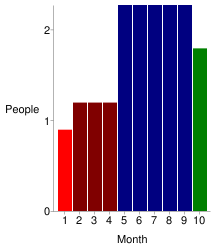
\includegraphics[scale=1.0]{chapters/cocomo_data/chart.png}
\caption{Staffing chart}
\end{figure}
